%______________________________________________________________________________
% T.Y. B.Tech. Project Report
% UWB Indoor RTLS + Digital Twin
% Format: Department of CSE, COEP Technological University, Pune
% Self-contained single-file source. Compile with: pdflatex (run 2-3 times for ToC).
%______________________________________________________________________________

\documentclass[a4paper,12pt,onecolumn]{report}

%______________________________________________________________________________
% Packages
%______________________________________________________________________________
\usepackage{graphicx}
% search these folders for figures, so \includegraphics resolves from any compile dir
\graphicspath{{./}{report/}{./report/}{../report/}%
  {TYProjects_Report_Format_2026-27/TYProjects_Report_Format_2025-26/}}
\usepackage{color}
\usepackage{float}
\usepackage{amsmath,amssymb}
\usepackage{booktabs}
\usepackage{longtable}
\usepackage{enumitem}
\usepackage{listings}
\usepackage[hidelinks]{hyperref}
\usepackage{url}

%______________________________________________________________________________
% Page Layout
%______________________________________________________________________________
\usepackage[left=2.5cm,top=2cm,right=2cm,bottom=2cm,bindingoffset=0.5cm]{geometry}
\setlength{\textwidth}{6.5in}
\setlength{\textheight}{9.5in}
\linespread{1.4}

% Listing style for JSON / code snippets
\definecolor{codegray}{gray}{0.95}
\lstset{
  basicstyle=\ttfamily\footnotesize,
  backgroundcolor=\color{codegray},
  breaklines=true,
  frame=single,
  captionpos=b,
  columns=fullflexible,
  showstringspaces=false
}

\begin{document}

%______________________________________________________________________________
% TITLE PAGE
%______________________________________________________________________________
\begin{titlepage}
\begin{center}
\LARGE{\bf{UWB Indoor Real-Time Location System with a Live 3D Digital Twin\\}}
\vspace{6pt}
\Large{\bf{ B. Tech. Project Report\\}}
\vspace{4pt}
\Large{\em{Submitted by\\}}
\begin{table}[htbp]
    \begin{center}
    \begin{tabular}{ l c c l }
    \Large\bf{Nahush Kale} & & & \Large\bf{612203081} \\[0.3cm]
    \Large\bf{Akshad Lohiya} & & & \Large\bf{612303104} \\[0.3cm]
    \Large\bf{Purnank Vasaikar} & & & \Large\bf{612303193} \\[0.3cm]
    \end{tabular}
    \end{center}
\end{table}

\Large{Under the guidance of\\ }
\Large{\bf{Prof. $<$Guide Name$>$}\\}
\begin{figure}[h]
\centering
\includegraphics[width=4cm,height=4cm]{TYProjects_Report_Format_2026-27/TYProjects_Report_Format_2025-26/COEP_Tech_University_Logo.jpg}
\end{figure}

\large{\bf{DEPARTMENT OF COMPUTER SCIENCE \& ENGINEERING}}\\
\Large{\bf{COEP TECHNOLOGICAL UNIVERSITY, PUNE-5}}
\vfill
\end{center}
\end{titlepage}

%______________________________________________________________________________
% CERTIFICATE
%______________________________________________________________________________
\thispagestyle{empty}
\linespread{1.6}
\begin{center}
\large{\bf{DEPARTMENT OF COMPUTER SCIENCE \& ENGINEERING,\\
      COEP TECHNOLOGICAL UNIVERSITY, PUNE-5\\}}
\end{center}

\vspace{12pt}
\begin{center}
\Large{\bf{CERTIFICATE\\}}
\end{center}
\vspace{12pt}

\linespread{1.5}\selectfont
\large{
Certified that the project titled, ``UWB Indoor Real-Time Location System with a
Live 3D Digital Twin'' has been successfully completed by \\
\begin{table}[htbp]
    \begin{center}
    \begin{tabular}{ l c c l }
    \Large\bf{Nahush Kale} & & & \Large\bf{612203081} \\ [0.3cm]
    \Large\bf{Akshad Lohiya} & & & \Large\bf{612303104} \\ [0.3cm]
    \Large\bf{Purnank vasaikar} & & & \Large\bf{612303193} \\ [0.3cm]
    \end{tabular}
    \end{center}
\end{table} \\
and is approved for the partial fulfillment of the requirements for the degree of
``B. Tech. Computer Science \& Engineering''.
}

\vspace{30pt}
\begin{center}
\normalsize{\bf{Dr. H.D. Gadade\hspace{\stretch{1}}Dr. P.K. Deshmukh\\
Project Guide\hspace{\stretch{1}}Head}\\
Department of CSE\hspace{\stretch{1}}Department of CSE\\
COEP Tech Pune,\hspace{\stretch{1}}COEP Tech Pune,\\
Shivajinagar, Pune - 5.\hspace{\stretch{1}}Shivajinagar, Pune - 5.}
\end{center}

%______________________________________________________________________________
% ABSTRACT
%______________________________________________________________________________
\newpage
\begin{center}
\Large \textbf{Abstract}
\end{center}
\addcontentsline{toc}{chapter}{Abstract}

Indoor asset and personnel tracking is a problem that GPS (blocked indoors) and
BLE / Wi-Fi (metre-to-tens-of-metre error) cannot solve reliably. This project
builds a cost-effective \textbf{Ultra-Wideband (UWB) Real-Time Location System
(RTLS)} that tracks tagged items to centimetre-to-decimetre accuracy inside a
warehouse-scale space and renders them moving live on a browser-based \textbf{3D
digital twin} of the floor. Ceiling-mounted UWB anchors (Makerfabs
MaUWB\_DW3000) range the tags using \textbf{DS-TWR (Double-Sided Two-Way
Ranging)}; a position engine converts those noisy ranges into a smooth track via
\textbf{weighted multilateration} followed by a \textbf{constant-velocity Kalman
filter}; and a React~+~Three.js dashboard visualises the labelled room, the
anchors, and every tag in real time with uncertainty and error-versus-truth
overlays.

The central engineering principle is \emph{one codebase, sim or hardware}: the
simulator and the (future) real hardware emit an identical, versioned data
format, so the entire downstream pipeline is developed and validated before any
hardware arrives, and hardware integration is reduced to a single drop-in file.
A key contribution is \textbf{data-driven NLOS (Non-Line-of-Sight) calibration}:
the range-noise and NLOS-bias model is fitted from the public, mm-ground-truth
\textbf{UTIL} UWB dataset, revealing that real NLOS error is a positive bias
($\approx$0.03--0.40~m), not merely added noise. On simulated LOS/NLOS data the
solver achieves $\approx$0.6--0.7~m median raw error; the Kalman filter adds
velocity, an uncertainty ellipse, and substantially smoother tracks. An optional,
walled-off \textbf{TDOA-EKF} module, validated directly against real UTIL
DWM1000 flight data, reaches $\approx$0.18--0.20~m 3D RMSE. The system is
verified by 21 automated tests and a live end-to-end demonstration.

%______________________________________________________________________________
% TOC / LISTS
%______________________________________________________________________________
\tableofcontents

\listoftables
\addcontentsline{toc}{chapter}{List of Tables}

\listoffigures
\addcontentsline{toc}{chapter}{List of Figures}

\chapter*{List of Abbreviations}
\addcontentsline{toc}{chapter}{List of Abbreviations}
\begin{longtable}{ l l }
\textbf{UWB}    & Ultra-Wideband \\
\textbf{RTLS}   & Real-Time Location System \\
\textbf{DS-TWR} & Double-Sided Two-Way Ranging \\
\textbf{TWR}    & Two-Way Ranging \\
\textbf{TDOA}   & Time-Difference-of-Arrival \\
\textbf{TOA}    & Time-of-Arrival \\
\textbf{LOS}    & Line-of-Sight \\
\textbf{NLOS}   & Non-Line-of-Sight \\
\textbf{WLS}    & Weighted Least Squares \\
\textbf{KF}     & Kalman Filter \\
\textbf{EKF}    & Extended Kalman Filter \\
\textbf{CV}     & Constant-Velocity (motion model) \\
\textbf{RMSE}   & Root-Mean-Square Error \\
\textbf{HUD}    & Heads-Up Display \\
\textbf{FP}     & First-Path (signal power) \\
\textbf{RX}     & Received (signal power) \\
\textbf{API}    & Application Programming Interface \\
\textbf{UTIL}   & UWB TDOA Indoor Localization dataset (UofT UTIAS DSL) \\
\end{longtable}

\newpage
\pagenumbering{arabic}

%==============================================================================
% CHAPTER 1 - INTRODUCTION
%==============================================================================
\chapter{Introduction}

\section{Background and Motivation}
Warehouses, hospitals, manufacturing floors and logistics hubs need to know
\emph{where} their assets and people are, indoors, in real time. Outdoors this is
solved by GPS, but GPS signals do not penetrate buildings, and the common indoor
alternatives---Wi-Fi and Bluetooth Low Energy (BLE) trilateration---suffer
metre-to-tens-of-metre errors because their signals are narrowband and highly
susceptible to multipath. \textbf{Ultra-Wideband (UWB)} radio transmits
extremely short pulses over a very wide bandwidth, which gives it fine temporal
resolution and strong multipath rejection, enabling \textbf{centimetre-to-decimetre}
ranging. This makes UWB the leading technology for high-accuracy indoor RTLS.

A location system is only useful if its output is legible. This project therefore
pairs the positioning engine with a \textbf{digital twin}---a live, labelled 3D
model of the physical floor---so operators can \emph{see} tagged items moving,
with zones, walls, and per-anchor signal quality rendered in the browser.

\section{Problem Statement}
Build an end-to-end, cost-effective indoor RTLS that (a) ranges tags from
ceiling anchors, (b) solves each tag's position from noisy, partially
Non-Line-of-Sight (NLOS) range measurements, (c) smooths the estimate over time,
and (d) visualises the result live in a 3D digital twin---while being
architected so the \emph{same software} runs against a realistic simulator today
and real UWB hardware tomorrow, with no downstream rewrites.

\section{Objectives}
\begin{enumerate}[nosep]
  \item Define a single, versioned data contract shared by the simulator and real
        hardware, so the two are interchangeable.
  \item Build a hardware-faithful UWB simulator that models DS-TWR ranging with
        realistic LOS/NLOS behaviour (wall occlusion, antenna-delay bias,
        positive-only NLOS bias, signal-power diagnostics, dropped readings).
  \item Implement a range-based \textbf{multilateration solver} that recovers
        position and \emph{down-weights} NLOS ranges using the DW3000 power gap.
  \item Fuse successive fixes with a \textbf{constant-velocity Kalman filter} to
        produce smooth tracks with velocity and an uncertainty estimate.
  \item Render a live, config-driven \textbf{3D digital twin} with trails,
        uncertainty rings, zone labels, and a live accuracy HUD.
  \item \textbf{Calibrate and validate} the noise/NLOS model against real,
        published UWB data with millimetre ground truth (the UTIL dataset).
  \item Keep hardware integration to a single drop-in source file.
\end{enumerate}

\section{Scope and Assumptions}
The deliverable targets a warehouse-scale single floor ($30\times30$~m in the
demo site) with four-to-five roughly co-planar ceiling anchors and a handful of
moving tags. The chosen hardware (MaUWB\_DW3000) performs DS-TWR and reports a
\emph{range per anchor} plus power diagnostics; it does not expose raw TDOA
timestamps, so the primary pipeline is \textbf{range-based}. Height ($y$)
observability is inherently weak with co-planar anchors, so the solver applies a
height-compensation assumption and can fall back to a fixed-height 2D solve.

\section{Organisation of the Report}
Chapter~2 surveys UWB positioning, NLOS mitigation and the reference dataset.
Chapter~3 presents the system architecture, data contracts and the shared site
configuration. Chapter~4 details the methodology and implementation of every
module. Chapter~5 reports results, accuracy and testing. Chapter~6 concludes and
lists future work.

%==============================================================================
% CHAPTER 2 - LITERATURE SURVEY
%==============================================================================
\chapter{Literature Survey}

\section{UWB Positioning Fundamentals}
UWB positioning estimates a tag's location from time measurements between the
tag and fixed anchors of known coordinates. Two dominant observation models
exist:
\begin{itemize}[nosep]
  \item \textbf{TWR / DS-TWR (range-based).} Each anchor--tag pair exchanges
        messages to directly measure a distance. \emph{Double-Sided} TWR sends
        an extra message so that device clock-drift terms cancel, which removes
        the need for anchor-to-anchor time synchronisation---a major practical
        simplification. Our hardware reports exactly this.
  \item \textbf{TDOA (time-difference-of-arrival).} The tag transmits once and
        anchors, \emph{sharing a synchronised clock}, compare arrival times; each
        anchor pair yields a hyperbola. This scales to many tags but needs tight
        anchor time-sync.
\end{itemize}

\section{The NLOS Problem}
When the direct (first) path between tag and anchor is blocked, the signal
arrives via reflection, so the measured range is reported \emph{longer} than the
true distance. Crucially, NLOS error is a \textbf{positive bias}, not a
zero-mean noise term, so it cannot be removed by simple averaging or filtering.
DW-family chips expose \textbf{received-signal power} and \textbf{first-path
power} registers; a large gap between them indicates an attenuated first path
and hence likely NLOS. This diagnostic is the key that our solver uses to detect
and down-weight NLOS measurements.

\section{Reviewed Literature}
Table~\ref{tab:litsurvey} summarises the primary references that shaped the
measurement model, NLOS handling and evaluation methodology.

\begin{table}[H]
\begin{center}
\begin{tabular}{ | p{4.3cm} | p{4.0cm} | p{4.7cm} | }
\hline
\multicolumn{3}{|c|}{\textbf{Table 2.1: Reviewed Literature}}\\
\hline
\textbf{Work} & \textbf{Focus} & \textbf{Relevance to this project}\\ \hline
Paszek et al., \emph{Sensors} 2021 --- UWB Positioning System Simulator for
LOS/NLOS &
Design of a UWB simulator; trilateration + ground-truth accuracy analysis &
Blueprint for a hardware-faithful LOS/NLOS simulator and for reporting accuracy
against ground truth \\ \hline
\emph{Appl. Sci.} 2025 (15-02689) --- NLOS-Exclusion Positioning &
Excluding/ down-weighting NLOS links; RMSE 0.124~m ($\approx$24\% improvement) &
Confirms NLOS-aware weighting as the highest-leverage accuracy lever \\ \hline
\emph{Appl. Sci.} 2024 (14-11005) --- UWB RTLS study &
Practical UWB RTLS deployment and error characterisation &
Deployment geometry and error-budget guidance \\ \hline
Zhao et al., IJRR 2024 --- \textbf{UTIL} dataset &
Raw UWB TDOA + SNR/power-difference + IMU + mm Vicon truth; DWM1000 &
Real-data source for NLOS/noise \emph{calibration} and for validating an EKF \\ \hline
\emph{Alexandria Eng. J.} 2018 (S1110016818) --- UWB localization &
Ranging/positioning error modelling &
Supporting error-model context \\
\hline
\end{tabular}
\caption{Summary of reviewed literature.}
\label{tab:litsurvey}
\end{center}
\end{table}

\section{Reference Dataset: UTIL}
The \textbf{UTIL} dataset (University of Toronto UTIAS Dynamic Systems Lab, IJRR
2024) is used as the real-data anchor of this project. It provides raw UWB TDOA
measurements, SNR and power-difference values labelled LOS/NLOS, IMU and
altitude data, and \textbf{millimetre-accurate Vicon ground truth} across four
anchor constellations and $\approx$150 minutes of flights, together with a
reference EKF and Python/MATLAB parsers. Its modules are Decawave \textbf{DWM1000}
--- the same DW-chip \emph{family} as our DW3000, but not identical, which
imposes a documented \textbf{cross-radio caveat}: the fitted model is a
\emph{prior} needing DW3000 recalibration, not a direct transplant.

%==============================================================================
% CHAPTER 3 - SYSTEM ARCHITECTURE AND DESIGN
%==============================================================================
\chapter{System Architecture and Design}

\section{High-Level Architecture}
The system is a three-stage pipeline behind a clean source interface
(Fig.~\ref{fig:arch}):
\[
\text{[Anchor Source]} \;\rightarrow\; \text{[Location Engine]} \;\rightarrow\;
\text{[Backend Hub]} \;\rightarrow\; \text{[Frontend Digital Twin]}
\]
The Anchor Source emits per-anchor \emph{ranges + power diagnostics}; the
Location Engine solves and filters position; the Backend is a thin Socket.IO
relay that also serves the site config; the Frontend is a pure visualiser of the
\emph{estimated} state.

\begin{figure}[H]
\begin{center}
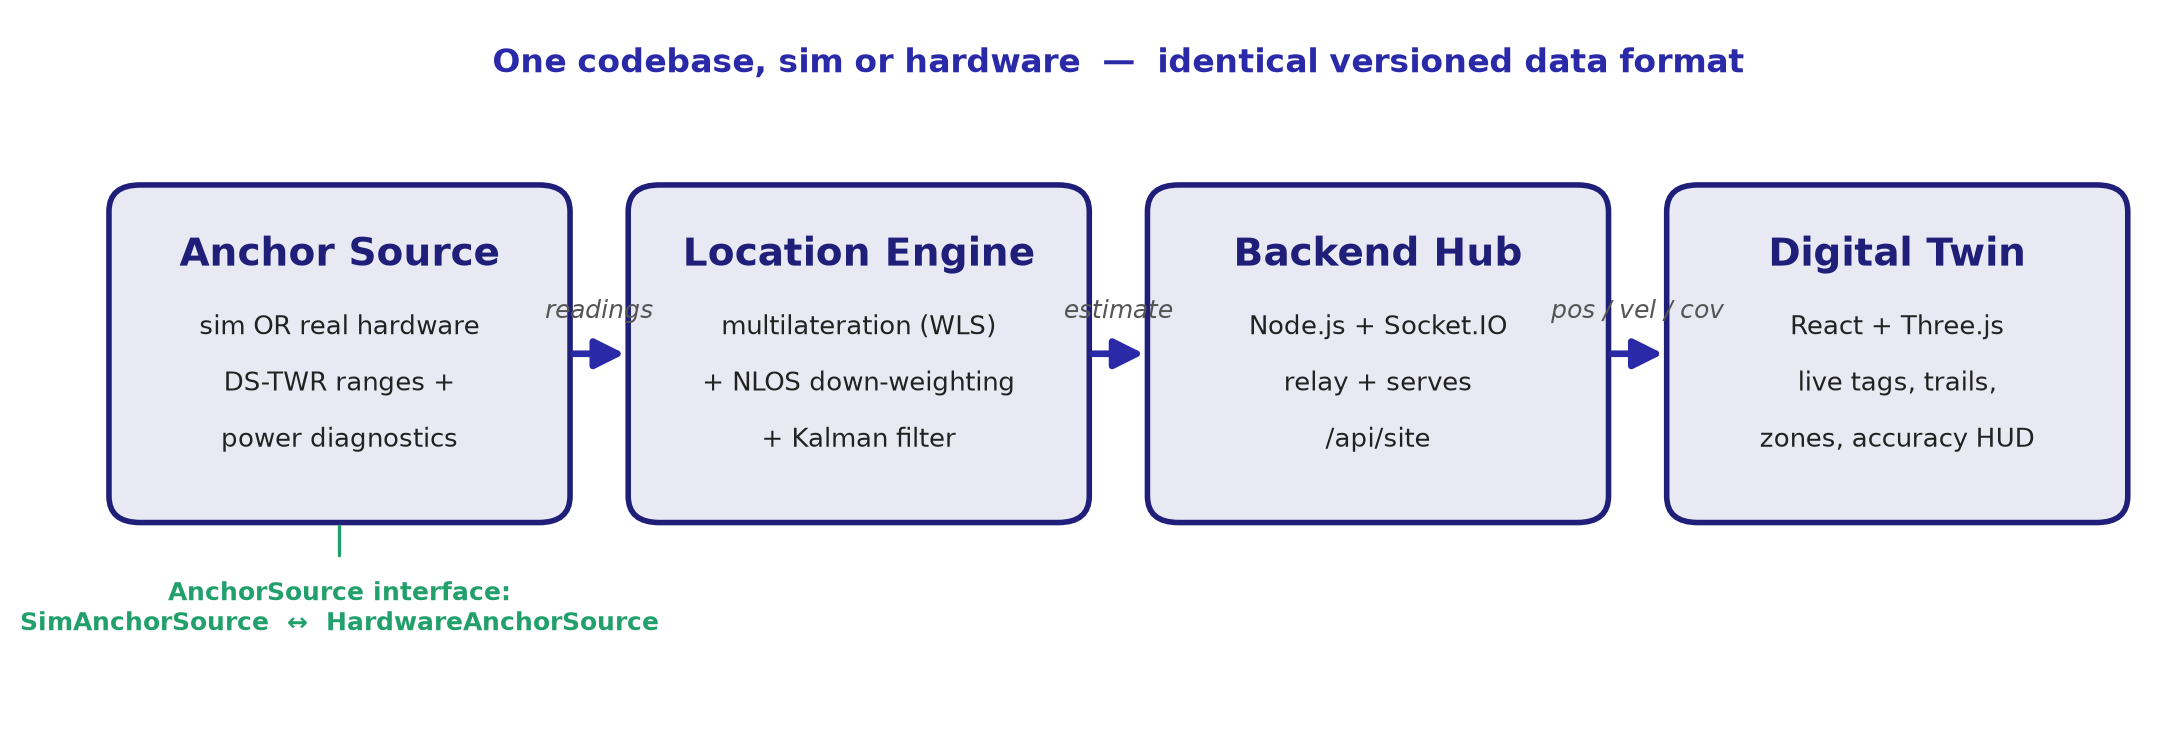
\includegraphics[width=\textwidth]{architecture.png}
\caption{Target architecture: a hardware-ready data source feeds a solve-and-filter
engine, relayed to a config-driven 3D twin. The \texttt{AnchorSource} interface lets
\texttt{SimAnchorSource} be swapped for \texttt{HardwareAnchorSource} with no
downstream change.}
\label{fig:arch}
\end{center}
\end{figure}

\section{The ``One Codebase, Sim or Hardware'' Principle}
The \texttt{AnchorSource} interface has two implementations selected by an
environment variable (\texttt{SOURCE=sim|hardware}): \texttt{SimAnchorSource}
(realistic UWB simulator) and \texttt{HardwareAnchorSource} (a UDP ingest seam
for the real MaUWB\_DW3000 nodes). Because both emit the identical versioned
data format, the location engine, backend and frontend are agnostic to the
source. Development and testing proceed fully before hardware arrives, and
hardware bring-up is confined to a single file.

\section{Class Design (UML)}
Figure~\ref{fig:uml} is the UML class diagram of the core pipeline, organised
into three layers. The \textbf{anchor sources} sit behind the abstract
\texttt{AnchorSource} interface: \texttt{SimAnchorSource} and
\texttt{HardwareAnchorSource} \emph{realise} it, while \texttt{DatasetTdoaSource}
and \texttt{TdoaSimulator} feed the walled-off TDOA track. The \textbf{data
model} is a small set of versioned carriers---\texttt{TagReading} (which
aggregates one \texttt{AnchorRange} per anchor) and \texttt{TdoaEvent}. The
\textbf{location engine} consumes those carriers: \texttt{LocationEngine}
composes one \texttt{ConstantVelocityKF} per tag and depends on the range
\texttt{solver} module for the weighted multilateration fix, while
\texttt{TdoaEKF} consumes \texttt{TdoaEvent}s for the real-data / generative TDOA
path. Because every source produces the same data model, swapping the simulator
for the hardware source leaves the engine and everything downstream untouched.

\begin{figure}[H]
\begin{center}
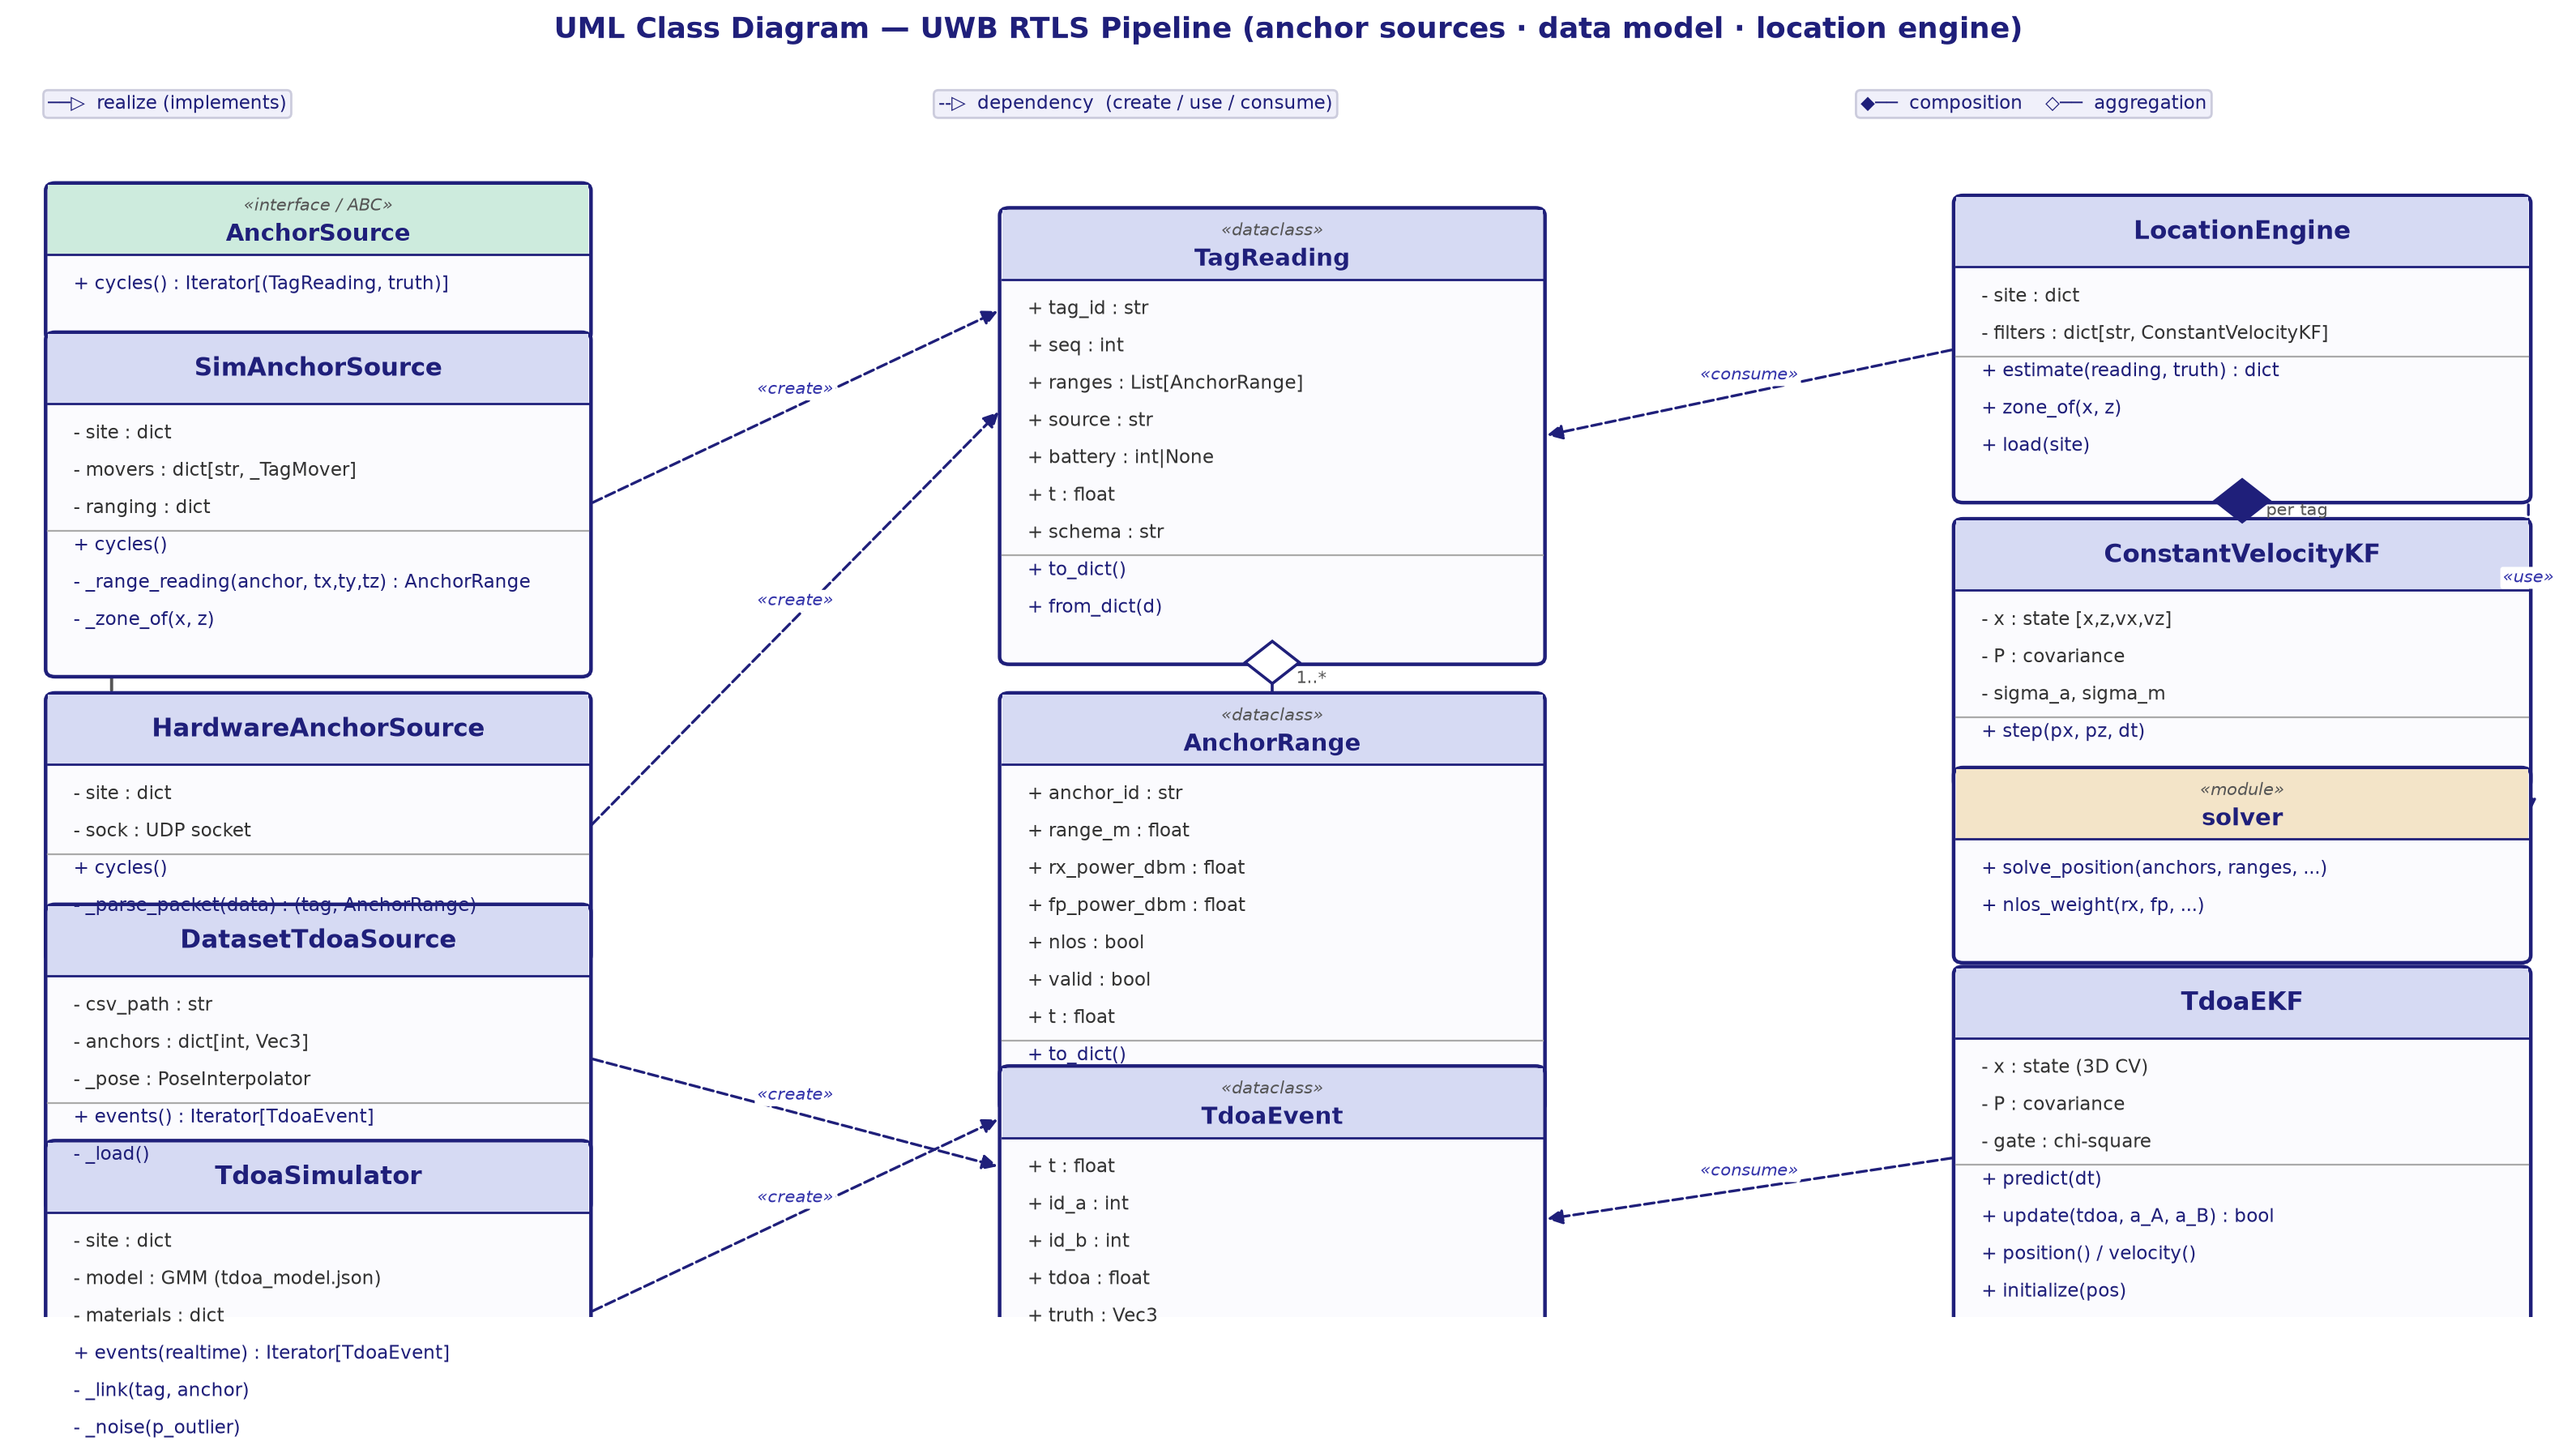
\includegraphics[width=\textwidth]{uml_class.png}
\caption{UML class diagram of the UWB RTLS pipeline: anchor sources (left), the
versioned data model (centre) and the location engine (right), showing realise,
dependency, composition and aggregation relationships.}
\label{fig:uml}
\end{center}
\end{figure}

\section{Data Contracts}
\subsection{Raw Measurement (source $\rightarrow$ engine)}
Schema \texttt{uwb.reading/1}: a per-anchor range with power diagnostics. The
\texttt{range} already includes real-world error (antenna-delay bias, Gaussian
noise, and under NLOS a positive-only excess bias). \emph{No ground truth}
reaches the solver.
\begin{lstlisting}[language=,caption={Raw reading schema (uwb.reading/1).}]
{ "schema":"uwb.reading/1", "tagId":"T1", "seq":1423, "source":"sim",
  "t":1757500000.12,
  "ranges":[ {"anchorId":"A1", "range":9.41, "rxPower":-83.2,
              "fpPower":-86.1, "nlos":false, "valid":true,
              "t":1757500000.11}, ... ] }
\end{lstlisting}

\subsection{Estimate (engine $\rightarrow$ backend $\rightarrow$ frontend)}
The engine emits filtered position, pre-Kalman raw fix (for comparison),
velocity, covariance (uncertainty ellipse), zone label, and---in simulation
only---the truth for the accuracy HUD.
\begin{lstlisting}[language=,caption={Estimate / location\_update payload.}]
{ "tagId":"Tag_A", "name":"Forklift", "battery":85, "floorId":"...",
  "pos":{"x":..,"y":..,"z":..}, "vel":{"vx":..,"vy":..,"vz":..},
  "cov":{"sx":..,"sz":..,"sxz":..},   // uncertainty ellipse
  "raw":{"x":..,"z":..},              // pre-Kalman multilateration
  "truth":{"x":..,"z":..},            // sim only - accuracy HUD
  "zone":"Aisle-2", "alerts":[] }
\end{lstlisting}

\section{Shared Site Configuration (the ``Labelled Map'')}
A single JSON file, \texttt{Model/config/site.json} (schema \texttt{uwb.site/1}),
is the single source of truth for both engine and frontend. It replaces
hardcoded coordinate lists and holds: anchor positions in metres, floor
dimensions, walls (with material), labelled zones (rectangles used for labelling
and geofencing), tag routes, and the ranging/noise model. Every value carries a
\textbf{provenance tag} (\texttt{guessed} / \texttt{measured} / \texttt{tested} /
\texttt{calibrated}) so the team knows what still needs on-site measurement.
Coordinates use \textbf{local metres} ($x$=east, $y$=up, $z$=north; origin at
floor centre)---standard and accurate for cm-scale indoor RTLS---replacing the
earlier GPS lat/lon scheme.

\begin{table}[H]
\begin{center}
\begin{tabular}{ | l | l | p{7.5cm} | }
\hline
\multicolumn{3}{|c|}{\textbf{Table 3.1: Key \texttt{site.json} sections}}\\
\hline
\textbf{Section} & \textbf{Example} & \textbf{Purpose}\\ \hline
\texttt{anchors} & A1--A5 at $y=4.6$~m & Known anchor coordinates + antenna-delay bias \\ \hline
\texttt{walls}   & racks (metal), walls (wood) & LOS occlusion + per-material NLOS \\ \hline
\texttt{zones}   & Dock, Aisle 1/2, Staging & Labelling + geofencing rectangles \\ \hline
\texttt{tags}    & Forklift, Worker, Pallet Jack & Routes, speed, allowed zones \\ \hline
\texttt{ranging} & DS-TWR, 5~Hz & Noise/NLOS/power model + Kalman tuning \\
\hline
\end{tabular}
\caption{Structure of the shared site configuration.}
\label{tab:site}
\end{center}
\end{table}

\section{Mapping Platform}
The dashboard doubles as a standalone indoor-mapping tool: a \textbf{map library}
(create/list/delete maps, each with an unguessable share key), a \textbf{2D
floor-plan editor} (draw walls, zones, place anchors, lay out tag routes), and a
\textbf{live 3D viewer} (\texttt{?map=KEY}). \emph{Save \& Apply} hot-reloads the
simulator, solver and 3D twin with no restart. Maps live in a backend store
(\texttt{Model/backend/maps/}) independent of the code; the gateway runs one map
at a time via \texttt{MAP=<key> python main.py}.

\section{Technology Stack}
\begin{table}[H]
\begin{center}
\begin{tabular}{ | l | l | }
\hline
\multicolumn{2}{|c|}{\textbf{Table 3.2: Technology stack}}\\
\hline
\textbf{Layer} & \textbf{Technology}\\ \hline
Anchor source / engine & Python 3.12, NumPy, SciPy (\texttt{least\_squares}) \\ \hline
Real-time transport & python-socketio, websocket-client / Socket.IO \\ \hline
Backend hub & Node.js, Express, Socket.IO \\ \hline
Frontend twin & React, Vite, Three.js \\ \hline
Testing & pytest (21 tests) \\ \hline
Hardware target & Makerfabs MaUWB\_DW3000 (DS-TWR firmware) \\
\hline
\end{tabular}
\caption{Technology stack by layer.}
\label{tab:stack}
\end{center}
\end{table}

%==============================================================================
% CHAPTER 4 - METHODOLOGY AND IMPLEMENTATION
%==============================================================================
\chapter{Methodology and Implementation}

\section{Anchor Source: Hardware-Faithful Simulator}
\texttt{SimAnchorSource} generates readings that match exactly what the DW3000
firmware emits, so the downstream pipeline cannot tell sim from hardware. Per
anchor, per tag, at 5~Hz it computes the true distance and then injects:
\begin{itemize}[nosep]
  \item \textbf{Antenna-delay bias} --- a fixed per-anchor offset.
  \item \textbf{Gaussian range noise} --- from the calibrated LOS $\sigma$.
  \item \textbf{LOS/NLOS decision} --- via a 2D wall-occlusion test
        (\texttt{geometry.py}); a blocked first path is flagged NLOS.
  \item \textbf{Positive-only NLOS bias} --- a blocked path is always reported
        \emph{longer}, with magnitude drawn per obstructing \emph{material}
        (metal racks bias more than wood).
  \item \textbf{Power diagnostics} --- \texttt{rxPower} and \texttt{fpPower}
        derived from distance and NLOS attenuation, reproducing the DW3000 gap.
  \item \textbf{Dropped readings} --- higher drop probability under NLOS.
\end{itemize}
Tag motion follows configured waypoint routes with per-waypoint pauses. Readings
are stamped with a \emph{simulated} clock so the downstream $dt$ is correct
regardless of real-time pacing.

\section{Location Engine: Range Multilateration Solver}
\texttt{solver.py} performs 2D trilateration with height compensation. Given
anchor positions $a_i$ and weighted ranges $r_i$, it minimises the weighted
range residual
\[
\min_{p}\; \sum_i w_i \left( \lVert p - a_i \rVert - r_i \right)^2
\]
using \texttt{scipy.optimize.least\_squares} (Levenberg--Marquardt), seeded from
the anchor centroid or the last known position. The weights $w_i$ implement
\textbf{NLOS down-weighting}: a large \texttt{rxPower $-$ fpPower} gap lowers a
link's weight so a biased (long) NLOS range cannot drag the fix. The solver was
verified to recover a known point to $<1$~cm on clean geometry, and to beat
naively trusting a biased anchor. \texttt{engine.py}'s
\texttt{LocationEngine.estimate(reading, truth)} wraps the solve, attaches the
zone, residual and error-vs-truth, and emits the \texttt{location\_update}
payload. It runs \emph{inside the gateway process}, matching how a real Pi
gateway would ingest and solve.

\section{Kalman Filter Fusion}
\texttt{kalman.py} implements a 2D \textbf{constant-velocity} Kalman filter with
state $[x, z, v_x, v_z]$. Each cycle it \emph{predicts} forward by $dt$ and
\emph{updates} with the solver's raw fix, outputting a smoothed position,
velocity and covariance. Process and measurement noise are tuned via the
\texttt{ranging.kalman} config block ($\sigma_{\text{process}}=2.0$,
$\sigma_{\text{meas}}=0.5$). One filter instance is kept per tag. The frontend
``Raw fix + uncertainty'' toggle shows the jittery raw ghost and its $2\sigma$
ring beside the smooth Kalman track. Because NLOS bias is \emph{systematic}, the
filter's headline error gain is modest ($\approx$4--5\%), but it delivers
velocity, an uncertainty ellipse, and much smoother, more usable tracks.

\section{Digital Twin (Frontend)}
The React~+~Three.js twin (Fig.~\ref{fig:twin}) is fully config-driven: it draws
the room, walls, labelled zones and anchors from \texttt{/api/site}, then renders
each tag live. Analytics layers include: fading \textbf{motion trails} of the
Kalman path (per-tag gradient) with an optional dashed \textbf{true-path}
overlay; a live \textbf{Accuracy HUD} showing running Kalman-vs-raw mean, median,
p90 and \% improvement plus a per-tag error sparkline; \textbf{uncertainty rings}
from the covariance; and \textbf{green/red anchor range lines} showing LOS vs
NLOS. The twin is interactive: clicking an anchor or tag opens a details panel,
and an \textbf{Edit Map} mode adds/removes/moves anchors and tags, persisted via
\texttt{PUT /api/site}; the backend broadcasts \texttt{site\_updated} and the
gateway + dashboard reload live.

\begin{figure}[H]
\begin{center}
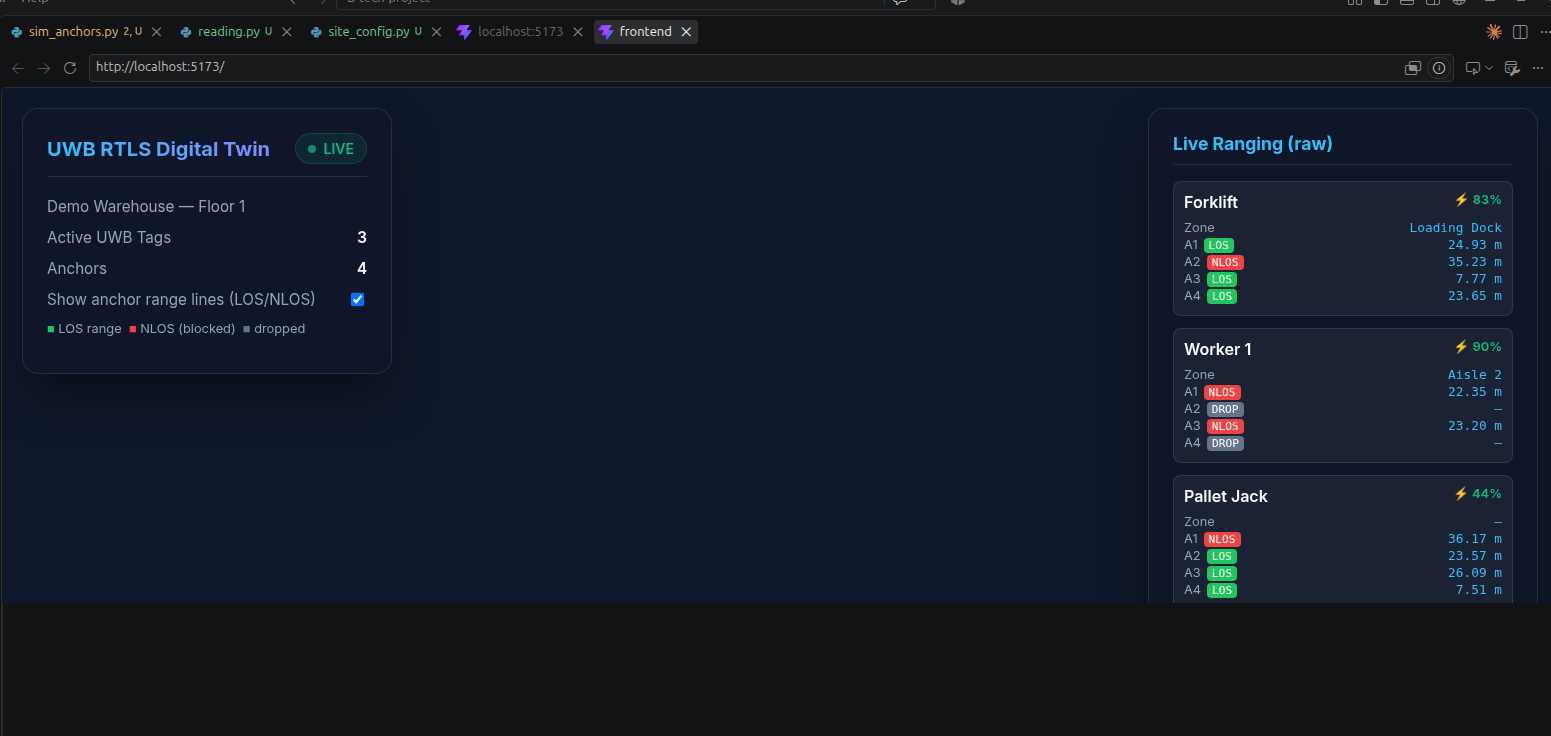
\includegraphics[width=0.9\textwidth]{twin screenshot.png}
\caption{The live 3D digital twin: labelled warehouse floor, anchors, zones and
tracked tags with anchor range lines.}
\label{fig:twin}
\end{center}
\end{figure}

\section{Data-Driven NLOS / Noise Calibration (UTIL)}
This is the highest-value use of real data. \texttt{calibrate\_from\_util.py}
derives real range-error statistics from UTIL's identification dataset---TDOA
truth from surveyed geometry, converting via
$\sigma_{\text{range}} = \sigma_{\text{tdoa}}/\sqrt{2}$---and patches the
\texttt{ranging} block of \texttt{site.json} (provenance becomes
\texttt{calibrated:UTIL-IJRR2024}). The calibration changed the model as shown in
Table~\ref{tab:calib}. The key empirical finding: \textbf{NLOS manifests as a
positive bias ($\approx$0.03--0.40~m), not extra noise}. Because
\texttt{SimAnchorSource} reads its model from config, this was a data change, not
a code change---so the simulator's injected noise now behaves like real DWM1000
UWB. The dBm power block was deliberately \emph{not} recalibrated (UTIL power
units are cross-radio; the WLS weight operates on our own consistent dBm gap).

\begin{table}[H]
\begin{center}
\begin{tabular}{ | l | c | c | }
\hline
\multicolumn{3}{|c|}{\textbf{Table 4.1: Effect of UTIL calibration}}\\
\hline
\textbf{Parameter} & \textbf{Before} & \textbf{After (calibrated)}\\ \hline
LOS noise $\sigma$ (m)      & 0.08 & \textbf{0.054} \\ \hline
NLOS noise $\sigma$ (m)     & 0.30 & \textbf{0.054} \\ \hline
NLOS bias min (m)           & 0.25 & \textbf{0.026} \\ \hline
NLOS bias max (m)           & 1.20 & \textbf{0.399} \\
\hline
\end{tabular}
\caption{Range-noise / NLOS-bias model before and after UTIL calibration.}
\label{tab:calib}
\end{center}
\end{table}

\section{Optional Walled-off Module: TDOA-EKF on Real Data}
To demonstrate an Extended Kalman Filter on real hardware-grade data---kept
\emph{off} the live warehouse critical path---the project includes a UTIL-only
TDOA track:
\begin{itemize}[nosep]
  \item \texttt{dataset\_source.py} --- \texttt{DatasetTdoaSource} replays a UTIL
        flight trial as a stream of \texttt{TdoaEvent}s. UTIL's CSV is a
        long-format event log whose pose column is not synced to the TDOA row, so
        ground truth is \textbf{interpolated to each TDOA timestamp} (raw pose
        gives 1.2~m error; interpolated $\approx$0.09~m).
  \item \texttt{ekf\_tdoa.py} --- \texttt{TdoaEKF}, a 3D constant-velocity EKF
        whose nonlinear measurement $h(p)=\lVert p-a_B\rVert-\lVert p-a_A\rVert$
        is linearised each step. A chi-square innovation gate rejects NLOS
        outliers; a Gauss--Newton cold start seeds the filter \emph{without}
        using ground truth. It also has a 2D fixed-height mode for near-coplanar
        ceiling anchors.
  \item \texttt{run\_tdoa\_ekf.py} --- benchmark runner; \texttt{test\_ekf\_tdoa.py}
        --- synthetic + real-trial tests (auto-skips if the dataset isn't extracted).
\end{itemize}

\section{Generative TDOA Simulator}
So that \emph{any} editable layout (not just the recording) can be driven by
TDOA+EKF, \texttt{train\_tdoa\_model.py} fits a 2-component Gaussian mixture
(inlier core + NLOS tail) to UTIL TDOA residuals via EM
($\sigma_{\text{inlier}}=0.137$~m, $\sigma_{\text{outlier}}=0.316$~m,
$p_{\text{outlier}}=0.11$) into \texttt{tdoa\_model.json}.
\texttt{sim\_tdoa.py}'s \texttt{TdoaSimulator} then yields TDOA events for a site
using the learned model plus geometry-aware NLOS (per-material). This runs live
at \texttt{?map=wh-tdoa} alongside the range-based \texttt{demo} and \texttt{util}
maps.

%==============================================================================
% CHAPTER 5 - RESULTS AND ANALYSIS
%==============================================================================
\chapter{Results and Analysis}

\section{Accuracy Results}
\begin{table}[H]
\begin{center}
\begin{tabular}{ | p{6.2cm} | c | p{4.5cm} | }
\hline
\multicolumn{3}{|c|}{\textbf{Table 5.1: Accuracy summary}}\\
\hline
\textbf{Configuration} & \textbf{Error} & \textbf{Notes}\\ \hline
Range solver, simulated LOS/NLOS & $\approx$0.6--0.7~m median raw & Weighted
multilateration \\ \hline
+ Constant-velocity Kalman & $\approx$4--5\% mean gain & Bias-limited; adds
velocity, covariance, smoothness \\ \hline
TDOA-EKF, real UTIL const1/const2 & $\approx$0.18--0.20~m 3D RMSE & Clean
constellations, vs mm Vicon \\ \hline
TDOA-EKF, real UTIL const3 & $\approx$0.33~m 3D RMSE & Cluttered; gate rejects
$\approx$3\% outliers \\ \hline
Generative TDOA sim on warehouse & $\approx$0.5~m horizontal RMSE & Learned model,
editable layout \\
\hline
\end{tabular}
\caption{Positioning accuracy across pipelines and data sources.}
\label{tab:accuracy}
\end{center}
\end{table}

\section{Discussion}
The results are internally consistent and literature-comparable. The
$\approx$0.6~m raw solver error on simulated data is dominated by the
\emph{systematic NLOS bias}, which is precisely why the constant-velocity Kalman
filter---excellent at attenuating zero-mean noise---yields only a modest headline
gain: it cannot remove a bias. This validates the plan-of-record decision to put
the highest-value effort into \textbf{NLOS-aware weighting and data-driven
calibration} rather than a heavier estimator. On real UTIL data, the TDOA-EKF's
0.18--0.33~m RMSE (degrading on the cluttered const3 as expected) confirms the
implementation is sound on hardware-grade measurements.

\section{Testing and Verification}
\textbf{Unit tests (pytest): 21 tests, all passing.} Coverage includes: the
solver recovering a known point to $<1$~cm and beating a biased anchor
(\texttt{test\_solver.py}); the Kalman filter reducing mean error on a noisy
known trajectory (\texttt{test\_kalman.py}); the calibration reproducing the
calibrated LOS $\sigma$ and positive-only NLOS bias (\texttt{test\_calibration.py});
the simulator's TDOA statistics (\texttt{test\_sim\_tdoa.py}); and the EKF on
synthetic and real trials (\texttt{test\_ekf\_tdoa.py}, real test auto-skips if
the dataset is absent).

\textbf{End-to-end:} starting backend, engine (sim source) and frontend confirms
tags tracked live, raw multilateration visibly jittering while the Kalman track
stays smooth, and the accuracy HUD showing filtered error below raw error.

\textbf{Hardware-readiness check:} the design confirms that swapping
\texttt{SimAnchorSource} $\rightarrow$ \texttt{HardwareAnchorSource} is the only
change needed to accept a real anchor feed---the engine is untouched.

\section{Implementation Status}
\begin{table}[H]
\begin{center}
\begin{tabular}{ | l | l | p{6.5cm} | }
\hline
\multicolumn{3}{|c|}{\textbf{Table 5.2: Phase completion status}}\\
\hline
\textbf{Phase} & \textbf{Status} & \textbf{Deliverable}\\ \hline
1. Foundation \& framework & \textbf{Done} & Site config, shared data format, simulator, config-driven twin \\ \hline
3. Range multilateration & \textbf{Done} & WLS solver + NLOS down-weighting; interactive Edit-Map \\ \hline
4. Kalman filter fusion & \textbf{Done} & Per-tag CV Kalman; velocity, covariance, raw-vs-filtered \\ \hline
5. Digital-twin upgrades & \textbf{Done} & Trails, true-path overlay, accuracy HUD, uncertainty rings \\ \hline
UTIL calibration & \textbf{Done} & Data-driven NLOS/noise model; \texttt{CALIBRATION.md} \\ \hline
TDOA-EKF (walled-off) & \textbf{Built} & Validated on real UTIL flights \\ \hline
Generative TDOA sim & \textbf{Built} & Learned model; runs on editable layouts \\ \hline
6. Basic AI (zones/predict) & \textbf{Pending} & Optional; geofence alerts + trajectory prediction \\
\hline
\end{tabular}
\caption{Phase-by-phase completion status.}
\label{tab:status}
\end{center}
\end{table}

%==============================================================================
% CHAPTER 6 - CONCLUSION AND FUTURE WORK
%==============================================================================
\chapter{Conclusion and Future Work}

\section{Conclusion}
This project delivers a complete, tested, hardware-ready indoor UWB RTLS with a
live 3D digital twin. The core pipeline---realistic DS-TWR simulator, weighted
multilateration solver with NLOS down-weighting, per-tag constant-velocity Kalman
filter, and a config-driven interactive twin---is fully implemented and
verified by 21 automated tests and an end-to-end live demonstration. The
distinctive contributions are (1) the \emph{one-codebase} architecture that makes
the simulator and real hardware interchangeable behind a single interface, and
(2) \emph{data-driven NLOS calibration} against the real, mm-ground-truth UTIL
dataset, which showed that NLOS error is a positive bias rather than added noise
and reshaped the simulator accordingly. An optional TDOA-EKF module, validated
directly on real DWM1000 flight data at $\approx$0.18--0.20~m RMSE, demonstrates
an Extended Kalman Filter on hardware-grade measurements without sitting on the
delivery critical path.

\section{Limitations}
\begin{itemize}[nosep]
  \item \textbf{Cross-radio gap:} the calibration is fitted on DWM1000; DW3000
        power registers, antenna and bandwidth differ, so the model is a prior
        needing on-hardware recalibration, not a transplant.
  \item \textbf{No in-situ ground truth:} without a warehouse Vicon equivalent,
        end-to-end accuracy on the real rig is not yet validated.
  \item \textbf{Weak height observability:} four roughly co-planar ceiling
        anchors make $z$ poorly observable; the solver compensates or falls back
        to fixed-height 2D.
  \item \texttt{HardwareAnchorSource} is currently a UDP stub pending physical
        hardware.
\end{itemize}

\section{Future Work}
\begin{enumerate}[nosep]
  \item \textbf{Phase 6 --- Basic AI:} geofence/zone anomaly detection (alert when
        an item leaves its allowed zone or goes stale) as the headline feature,
        plus near-free short-horizon trajectory prediction ($p + v\,\Delta t$
        ``ghost'' marker) reusing the Kalman velocity state.
  \item \textbf{Hardware bring-up:} implement \texttt{HardwareAnchorSource} for
        the real MaUWB\_DW3000 feed and re-tune the noise/power model on DW3000.
  \item \textbf{In-situ validation:} collect tape-measured, NLOS-labelled DS-TWR
        traces on the real rig to confirm the calibration transfer direction.
  \item \textbf{Anchor geometry:} add more, better-spread anchors to improve
        height observability and overall accuracy.
\end{enumerate}

%______________________________________________________________________________
% REFERENCES
%______________________________________________________________________________
\begin{thebibliography}{9}
\addcontentsline{toc}{chapter}{References}

\bibitem{paszek2021}
K. Paszek, D. Grzechca, and A. Becker,
``Design of the UWB Positioning System Simulator for LOS/NLOS Environments,''
\emph{Sensors}, vol. 21, no. 14, 4757, 2021.

\bibitem{applsci2025}
``NLOS-Exclusion Based UWB Positioning Algorithm,''
\emph{Applied Sciences}, vol. 15, 02689, 2025.

\bibitem{applsci2024}
``UWB Real-Time Location System Study,''
\emph{Applied Sciences}, vol. 14, 11005, 2024.

\bibitem{util2024}
W. Zhao, A. Goudar, X. Qiao, and A. P. Schoellig,
``UTIL: An Ultra-wideband Time-difference-of-arrival Indoor Localization Dataset,''
\emph{Int. Journal of Robotics Research (IJRR)}, 2024.
Available: \url{https://utiasdsl.github.io/util-uwb-dataset/}

\bibitem{alexandria2018}
``UWB Indoor Localization Error Modelling,''
\emph{Alexandria Engineering Journal}, S1110016818302151, 2018.

\bibitem{makerfabs}
Makerfabs, ``MaUWB\_DW3000 UWB Module (ESP32 + DW3000, DS-TWR firmware).''
Product documentation.

\end{thebibliography}

\end{document}
